\documentclass[../main.tex]{subfiles}

\begin{document}

\section{Methodology}
\justify

This section describes the research design and all practical steps taken to answer the three research questions. It covers the overall experimental strategy, the simulation environment, the PPO training pipeline \cite{Schulman2017}, the physical drone platform, and the evaluation protocol used in both simulation and real-world trials.

\subsection{Research Design}

\subsubsection{Overview}

This study adopts a quantitative experimental design. The goal is to measure, under controlled and reproducible conditions, whether a PPO agent trained exclusively on monocular camera observations in simulation can perform effective obstacle avoidance in a real forest environment. Two experimental phases are used: a simulation training plus evaluation phase and a real-world validation phase.

\subsubsection{Variables}

The independent variables are tree count and density. The dependent variables are obstacle avoidance success rate, collision rate, and goal reached. All other factors --- drone hardware, camera parameters, control frequency, weather conditions, drone speed and cruise altitude --- are treated as control variables and held constant across conditions. Table \ref{tab:variables} summarises all three variable categories.

This design allows direct comparison between simulation and real-world performance, and supports a quantitative answer to whether PPO-based vision-only navigation is viable for forest monitoring applications.

\begin{table}[H]
    \small
    \centering
    \vspace*{\baselineskip}
    \caption{Independent, dependent, and control variables. Logged identically in simulation and in the real-world flights.}
    \label{tab:variables}
    \begin{tabular}{p{3cm} p{4cm} p{6cm}}
        \hline\hline
        \rowcolor{lightgray}\textbf{Variable type} & \textbf{Variable} & \textbf{Values / Range} \\\hline
        Independent & Tree density & Sparse (2 trees) / Dense (3 trees) \\
        \rowcolor{lightlightgray} Independent & Environment & Simulation / Real forest \\
        Dependent & Trees avoided & 0--3 (per episode) \\
        \rowcolor{lightlightgray} Dependent & Episode result & Success / Fail \\
        Dependent & Avoidance rate & Trees avoided / Trees in corridor $\times$ 100 \\
        \rowcolor{lightlightgray} Dependent & Success rate & Successful episodes / Total episodes $\times$ 100 \\
        Dependent & Sim-to-real ratio & Real success rate / Sim success rate (per density) \\
        \rowcolor{lightlightgray} Control & Forward cruise speed & 1.0\,m/s \\
        Control & Lateral avoidance speed & 2.0\,m/s \\
        \rowcolor{lightlightgray} Control & Cruise altitude & 1.5\,m \\
        Control & Camera FOV & 62$^{\circ}$ \\
        \rowcolor{lightlightgray} Control & Camera resolution & 126$\times$224\,px \\
        Control & Control frequency & $\sim$10\,Hz \\
        \rowcolor{lightlightgray} Control & Weather conditions & Wind $<$ 3\,m/s, daylight, no precipitation \\
        \hline
    \end{tabular}
\end{table}


\subsection{Simulation}

\subsubsection{Training in a simulation --- The environment}

All training and evaluation was conducted in \textit{Cosys-AirSim}, a community-maintained fork of \textit{Microsoft AirSim}, running on \textit{Unreal Engine 5.5}. \textit{Cosys-AirSim} was chosen specifically because it exposes runtime object manipulation APIs, \texttt{simSetObjectPose} and \texttt{simSetObjectScale}, which allow tree positions and scales to be updated between episodes without reloading the scene. The simulator provides a high-fidelity physics engine, realistic aerodynamic modelling, and configurable realistic sensor readings \cite{Kabas2022,Loquercio2019}, and the drone model closely matches the physical \textit{Holybro S500 V2} platform used in real-world trials. Figure \ref{fig:airsim_env} demonstrates how realistic the simulated drone environment looks.

The forest environment is built from Unreal Engine static mesh trees textured with realistic tree assets. Using a texture pack means the agent is trained on a visually consistent trunk appearance, an intentional simplification consistent with domain randomisation strategies reported in the literature \cite{Loquercio2019,Jang2024}, keeping the visual domain focused on trunk geometry rather than species-specific bark detail. (Figure \ref{fig:texture_pack})

\begin{figure}[H]
    \centering
    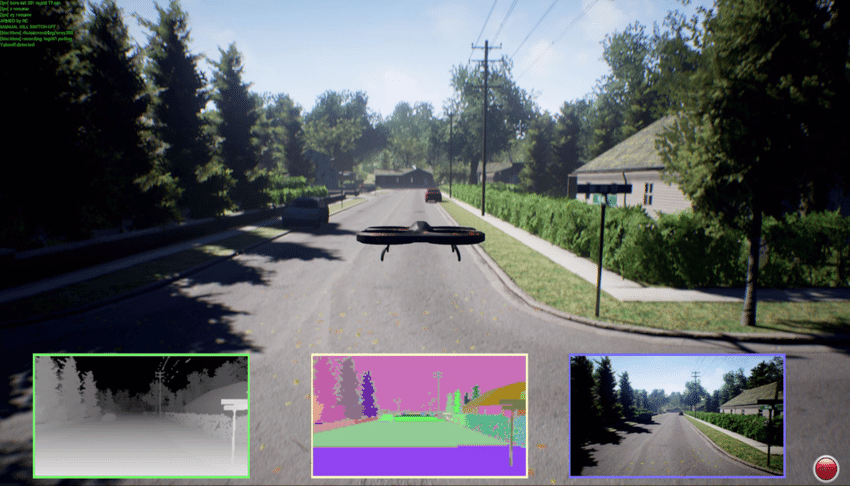
\includegraphics[width=0.75\textwidth]{figures/airsim_env.png}
    \caption{Demonstration of the Cosys-AirSim simulation environment used for training and evaluation. Source: \url{https://www.researchgate.net/figure/Airsim-Simulator-images-with-a-drone12_fig3_363486862}}
    \label{fig:airsim_env}
\end{figure}

\begin{figure}[H]
    \centering
    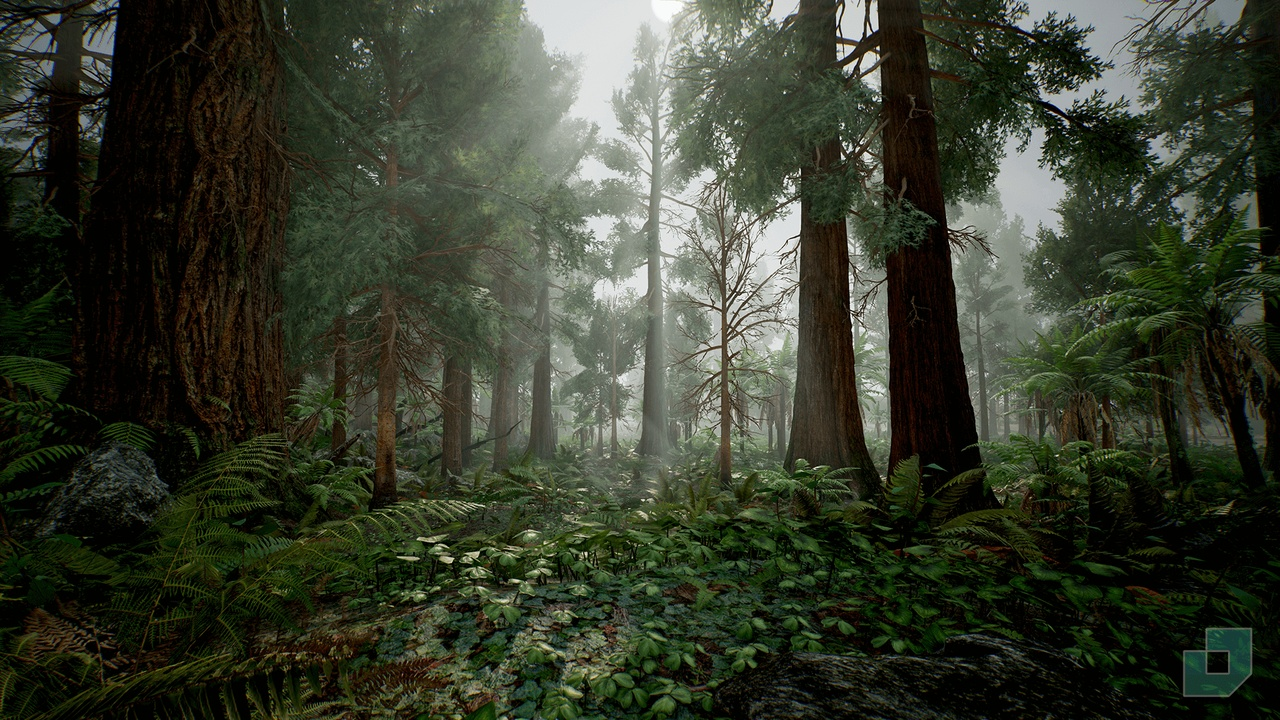
\includegraphics[width=0.75\textwidth]{figures/texture_pack.png}
    \caption{Example image of the redwood forest texture pack used in the simulation. Source: \url{https://www.fab.com/listings/a9135a3b-ce12-4648-88df-b84b1445de8a}}
    \label{fig:texture_pack}
\end{figure}

With the environment in place, the next step is defining how each training episode runs inside it.

\subsubsection{Training in a simulation --- The curriculum}

Each training episode begins with the drone spawning at a fixed position and a goal placed exactly 15 metres ahead.

The curriculum consists of three stages that vary tree density, size, and spacing rather than distance, since obstacle avoidance is a local skill that does not depend on how far the goal is.

Stage 1 uses sparse small trees with an average spacing of 6 metres and a cap of 8 trees, giving the agent room to learn basic lateral corrections.

Stage 2 increases density to one tree every 4 metres with up to 12 trees of medium size, forcing the agent to make faster decisions.

Stage 3 places up to 20 trees at 2-metre average spacing with varied scales, representing a dense forest corridor.

All trees are constrained to a 6-metre-wide corridor aligned with the spawn-to-goal axis, ensuring obstacles are always in the drone's path.

A 2-metre spawn clearance is enforced so the drone always takes off into open space.

Remaining tree assets are placed outside the corridor but within the flight radius to maintain visual realism for better generalisation of the training without interfering with the avoidance task.

The curriculum is intentionally randomised to support domain randomisation \cite{Zhao2020,Salvato2021,Loquercio2019}. Lighting conditions are varied during training by simulating different times of day, which alters sun position and changes the appearance of the environment across episodes.

In addition, the stage progression is random each episode, exposing the agent to all difficulty stages (Stages 1, 2, and 3) throughout training.

The stages and all other details mentioned in this section are shown in Figures \ref{fig:lighting_variation} to \ref{fig:stage_views}.

\begin{figure}[H]
    \centering
    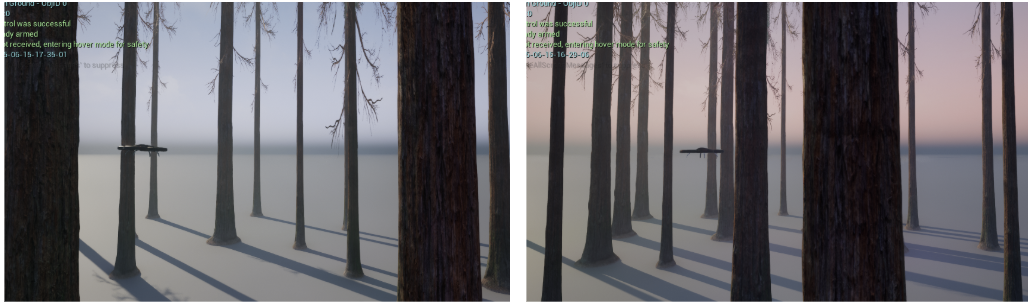
\includegraphics[width=0.75\textwidth]{figures/lighting_variation.png}
    \caption{The drone operates under different random lighting positions.}
    \label{fig:lighting_variation}
\end{figure}

\begin{figure}[H]
    \centering
    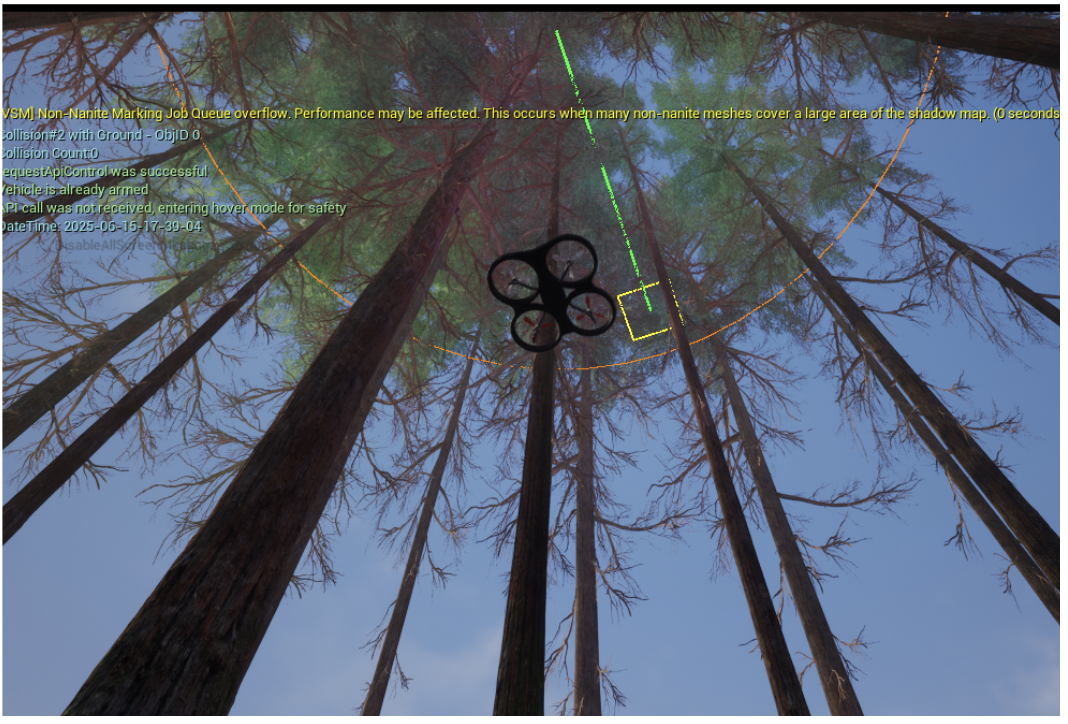
\includegraphics[width=0.75\textwidth]{figures/goal_view.png}
    \caption{View below the drone with a marked yellow square as the goal, the green line is the optimal path and the orange circle is the area where the goal can be randomly placed.}
    \label{fig:goal_view}
\end{figure}

\begin{figure}[H]
    \centering
    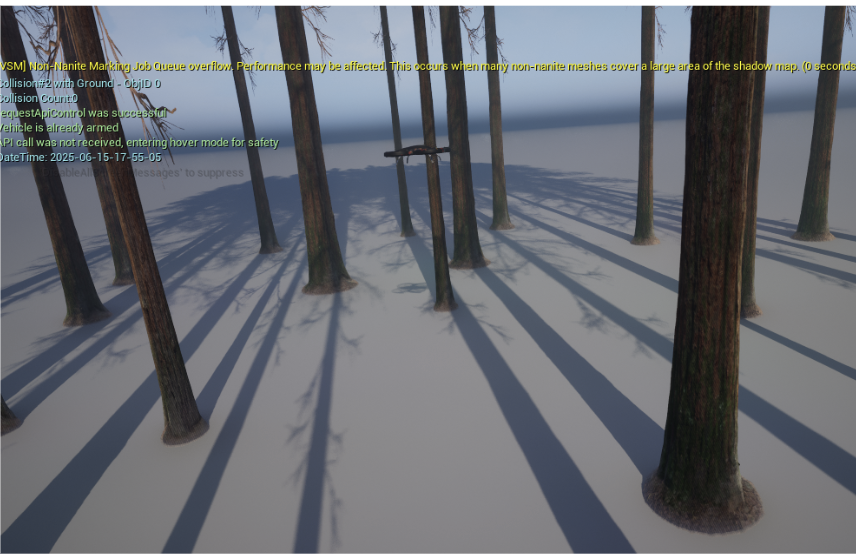
\includegraphics[width=0.75\textwidth]{figures/spawn_clearance.png}
    \caption{The trees are spawned while maintaining a 2\,m clearance for the spawned drone to start manoeuvring.}
    \label{fig:spawn_clearance}
\end{figure}

\begin{figure}[H]
    \centering
    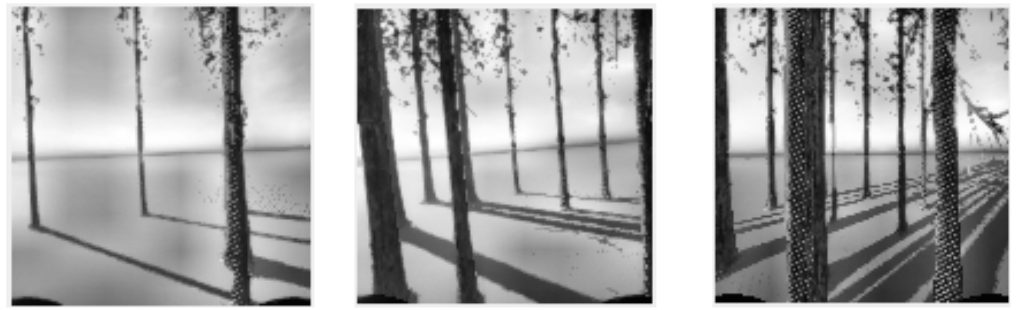
\includegraphics[width=0.95\textwidth]{figures/stage_views.png}
    \caption{The simulated drone's view of Stage 1 (6\,m average tree spacing, left), Stage 2 (4\,m average tree spacing, centre), and Stage 3 (2\,m average tree spacing, right).}
    \label{fig:stage_views}
\end{figure}

\subsubsection{Training in a simulation --- The sensor setup}

The drone sees the world through a single forward-facing camera capturing 128 $\times$ 128 pixel images at 30\,Hz with a 100\textdegree{} field of view, the same resolution, frame rate, and angle as the Arducam IMX477 mounted on the physical drone, ensuring no sensor mismatch between simulation and reality. Matching simulation and physical sensor parameters is a standard practice for minimising the reality gap \cite{Zhao2020,Salvato2021,Loquercio2019}.

Each raw colour frame goes through three processing steps before it reaches the network.

First, it is converted to grayscale, removing colour information the agent does not need and reducing sensitivity to lighting differences between simulation and the real world \cite{Loquercio2019}. (Figure \ref{fig:grayscale})

Second, CLAHE (Contrast Limited Adaptive Histogram Equalisation) is applied, enhancing local contrast so that dark tree trunks stand out against bright sky backgrounds regardless of overall scene brightness. (Figure \ref{fig:clahe})

Third, a small amount of Gaussian noise is added to replicate the sensor noise present in real camera images; injecting noise during training is a form of domain randomisation that prevents the agent from overfitting to the clean images a simulator produces \cite{Zhao2020,Salvato2021,Loquercio2019}. (Figure \ref{fig:gaussian_noise})

\begin{figure}[H]
    \centering
    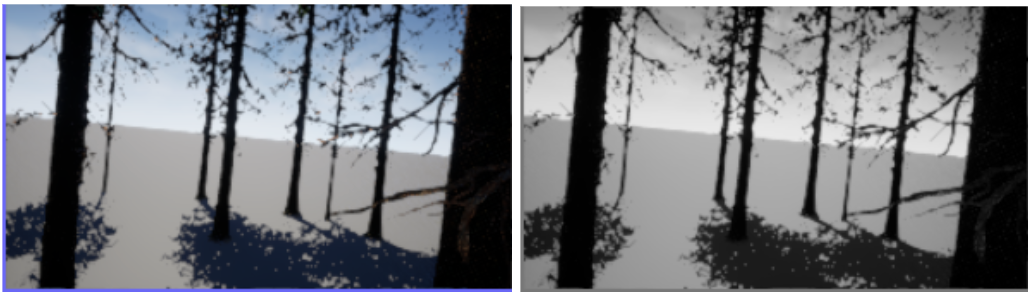
\includegraphics[width=0.75\textwidth]{figures/grayscale.png}
    \caption{Raw colour image captured by the simulated camera and the grayscale conversion of the raw camera frame.}
    \label{fig:grayscale}
\end{figure}

\begin{figure}[H]
    \centering
    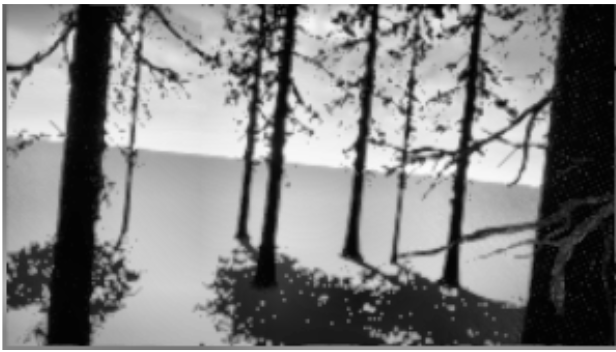
\includegraphics[width=0.60\textwidth]{figures/clahe.png}
    \caption{Frame after CLAHE preprocessing, showing enhanced local contrast.}
    \label{fig:clahe}
\end{figure}

\begin{figure}[H]
    \centering
    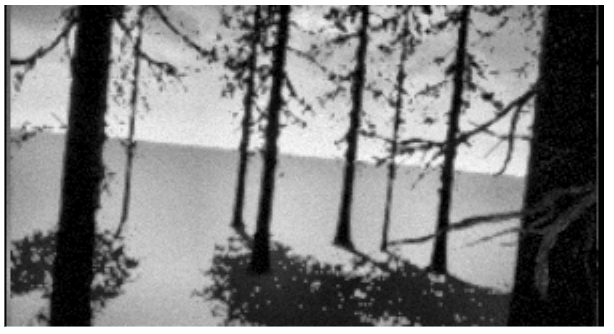
\includegraphics[width=0.60\textwidth]{figures/gaussian_noise.png}
    \caption{Frame after CLAHE preprocessing plus added Gaussian noise.}
    \label{fig:gaussian_noise}
\end{figure}

\subsubsection{Training in a simulation --- Observation and action states}

The drone observes (observation space) an 8-frame stack of converted grayscale camera images (128 $\times$ 128) so it can sense motion, plus a small 4-number state vector telling it how far the goal is, how far off-centre it is, and its current forward and lateral speeds.

With this observation space, the drone outputs two values: how much to dodge left or right (up to $\pm$1.5\,m/s), and how fast to fly forward (between 0.4 and 0.75\,m/s). (Table \ref{tab:obs_action})

\begin{table}[H]
    \small
    \centering
    \caption{Observation and action space.}
    \label{tab:obs_action}
    \begin{tabular}{p{3cm} p{3cm} p{5cm} p{3.5cm}}
        \hline\hline
        \rowcolor{lightgray}\textbf{Space} & \textbf{Component} & \textbf{Description} & \textbf{Range / Shape} \\\hline
        Observation Space & Visual input & 8-frame grayscale stack & 8 $\times$ 128 $\times$ 128 pixels \\
        \rowcolor{lightlightgray} & State vector & Goal distance, lateral offset, forward speed, lateral speed & 4 scalar values \\
        Action Space & Lateral velocity & Left/right dodge & $\pm$1.5\,m/s \\
        \rowcolor{lightlightgray} & Forward velocity & Forward flight speed & 0.4 -- 0.75\,m/s \\
        \hline
    \end{tabular}
\end{table}


\subsubsection{Training in a simulation --- Reward system}

The reward function combines dense shaping terms that guide the agent continuously with sparse terminal signals that mark clear success or failure. Table \ref{tab:reward} lists every component.

The progress term (+25 per metre) provides dense feedback that continuously incentivises forward movement toward the goal.

The time penalty ($-$0.2 per step) discourages hovering and inefficient paths.

A soft lateral offset penalty is applied proportionally when the drone drifts more than 0.5\,m perpendicular to the spawn-to-goal axis, encouraging the policy to stay on course.

A goal bonus of $+$100 is awarded on successful arrival, supplemented by an efficiency bonus of up to $+$20 that scales with how quickly the episode was completed relative to the step budget.

A uniform collision penalty of $-$50 terminates the episode immediately on physical contact with any tree.

A timeout penalty of $-$20 is applied if the drone fails to reach the goal within the allocated step budget.

All rewards are normalised online using VecNormalize to keep the signal stable across the three curriculum stages.

\begin{table}[H]
    \small
    \centering
    \caption{The model's reward system used in the curriculum.}
    \label{tab:reward}
    \begin{tabular}{p{4.5cm} p{5cm} p{3cm}}
        \hline\hline
        \rowcolor{lightgray}\textbf{Component} & \textbf{Condition} & \textbf{Value} \\\hline
        Progress reward & Per metre closed to goal & $+$25 \\
        \rowcolor{lightlightgray} Time penalty & Per timestep & $-$0.2 \\
        Lateral offset penalty & Offset $>$ 0.5\,m from path & Proportional ($-$0.3/m) \\
        \rowcolor{lightlightgray} Goal bonus & Goal waypoint reached & $+$100 \\
        Efficiency bonus & Goal reached quickly & Up to $+$20 \\
        \rowcolor{lightlightgray} Collision & Physical contact with tree & $-$50 \\
        Timeout & Max steps exceeded & $-$20 \\
        \hline
    \end{tabular}
\end{table}


\subsubsection{Training in a simulation --- The model network}

The actor uses a dual-stream network that processes the two inputs separately before combining them.

The visual stream uses a CNN to process the 8-frame grayscale stack, as mentioned in Section 2.2.4, producing a compact visual summary.

The state stream uses a small 4-element state vector to process the scalar flight values.

Both outputs are concatenated and fed into policy and value heads trained end-to-end using PPO \cite{Schulman2017}.

The critic network uses a larger value head of two fully connected layers of 128 units, giving it more capacity than the policy head to estimate returns across the varied difficulty stages.

\subsubsection{Preparation --- The model hyperparameters}

The model's network consists of the hyperparameters shown in Table \ref{tab:hyperparameters}.

\begin{table}[H]
    \small
    \centering
    \caption{The model's hyperparameters used in the curriculum.}
    \label{tab:hyperparameters}
    \begin{tabular}{p{6cm} p{6cm}}
        \hline\hline
        \rowcolor{lightgray}\textbf{Hyperparameter} & \textbf{Value} \\\hline
        Algorithm & PPO \\
        \rowcolor{lightlightgray} Learning rate & $1\times10^{-4}$ \\
        Rollout steps (n\_steps) & 8192 \\
        \rowcolor{lightlightgray} Minibatch size & 256 \\
        Epochs per update & 8 \\
        \rowcolor{lightlightgray} Discount factor ($\gamma$) & 0.97 \\
        GAE lambda ($\lambda$) & 0.95 \\
        \rowcolor{lightlightgray} Entropy coefficient & 0.01 \\
        Value function coefficient & 0.75 \\
        \rowcolor{lightlightgray} Max gradient norm & 0.5 \\
        Reward normalisation & VecNormalize (online) \\
        \rowcolor{lightlightgray} Device & CUDA (GPU) \\
        \hline
    \end{tabular}
\end{table}


\subsubsection{Testing in a simulation --- Results}

Evaluation is conducted separately under fixed, controlled conditions identical between simulation and the real world, allowing direct performance comparison. The curriculum and its randomisation are not active during evaluation.

The best policy checkpoint was evaluated over 50 episodes per configuration. Conditions are defined by tree spacing: sparse (6\,m, stage 1), medium (4\,m, stage 2), and dense (2\,m, stage 3), combined with a fixed speed within range of 0\,m/s as a minimum and 3\,m/s as a maximum. An episode was counted as successful if and only if the drone reached the goal waypoint without any collision and without leaving the defined corridor ($\pm$3\,m lateral hard kill) \cite{Kabas2022}. The goal distance for the simulation testing corridor, like in training, is 15\,m in length. The testing data structure is shown in Table \ref{tab:data_structure}.

\begin{table}[H]
    \small
    \centering
    \caption{Real-world and simulation testing data structure, one row per flight.}
    \label{tab:data_structure}
    \begin{tabular}{p{3.5cm} p{2.5cm} p{7cm}}
        \hline\hline
        \rowcolor{lightgray}\textbf{Column} & \textbf{Type} & \textbf{Description} \\\hline
        episode\_id & String & Unique identifier \\
        \rowcolor{lightlightgray} environment & Categorical & Real\_world or Simulation \\
        tree\_distance & Integer & Measured average tree distance before session (2\,m, 4\,m, 6\,m) \\
        \rowcolor{lightlightgray} brightness\_lux & Integer & Measured at flight time with a light meter in lux (Real\_world); approximate lighting in lux (Simulation) \\
        trees\_avoided & Integer & Trees passed without physical contact (Simulation and Real\_world) or without requiring RC failsafe operation (Real\_world) \\
        \rowcolor{lightlightgray} collision\_occurred & Boolean & True if IMU accelerometer spike exceeds threshold (Real\_world) or drone crashed and episode terminated (Simulation) \\
        goal\_reached & Boolean & True if the intended goal waypoint was reached \\
        \rowcolor{lightlightgray} time & Float & Flight time before collision\_occurred or goal\_reached \\
        success & Boolean & goal\_reached AND NOT collision\_occurred \\
        \hline
    \end{tabular}
\end{table}


\subsection{Real-World}

\subsubsection{Preparation --- The hardware setup}

The physical drone used for real-world evaluation was a \textit{Holybro S500 V2} quadcopter (500\,mm wheelbase) with a total all-up weight of approximately 1.75\,kg. The flight controller was a Pixhawk 6C running PX4 firmware v1.14+, operating in altitude control mode. The companion computer was an NVIDIA Jetson Orin Nano (8\,GB), selected for its ability to run TensorRT-optimised inference in real time \cite{Kabas2022}. The camera was an Arducam IMX477 configured to match the simulation sensor parameters exactly: 128 $\times$ 128 pixels, 30\,fps, 100\textdegree{} FOV, following the sensor-matching approach recommended for sim-to-real transfer \cite{Zhao2020,Salvato2021}. Figure \ref{fig:drone_hardware} shows how the setup looks in real life and Table \ref{tab:hardware} lists the key components of the setup.

\begin{figure}[H]
    \centering
    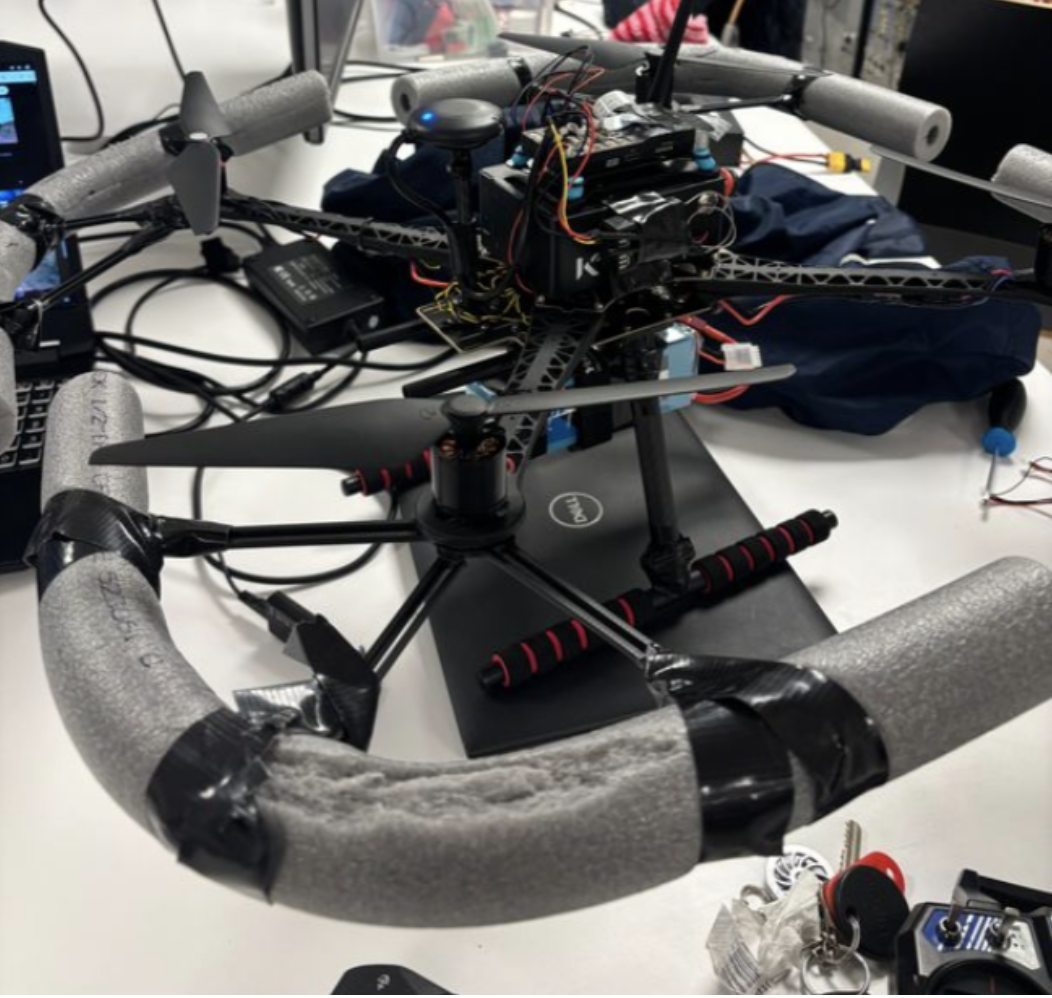
\includegraphics[width=0.65\textwidth]{figures/drone_hardware.png}
    \caption{The Holybro S500 V2 quadrotor used for real-world evaluation, equipped with the Arducam IMX477 camera, Pixhawk 6C flight controller, and NVIDIA Jetson Orin Nano companion computer.}
    \label{fig:drone_hardware}
\end{figure}

\begin{table}[H]
    \small
    \centering
    \caption{Physical drone hardware components.}
    \label{tab:hardware}
    \begin{tabular}{p{4cm} p{9cm}}
        \hline\hline
        \rowcolor{lightgray}\textbf{Component} & \textbf{Specification} \\\hline
        Frame & Holybro S500 V2 (500\,mm wheelbase) \\
        \rowcolor{lightlightgray} Flight controller & Pixhawk 6C, PX4 firmware v1.14+ \\
        Companion computer & NVIDIA Jetson Orin Nano (8\,GB) \\
        \rowcolor{lightlightgray} Camera & Arducam IMX477, 100\textdegree{} FOV, 128$\times$128 @ 60\,fps (tuned to 30\,fps) \\
        GPS & Holybro M10 GPS module \\
        \rowcolor{lightlightgray} Telemetry & 433\,MHz SiK radio \\
        Battery & 4S 5000\,mAh LiPo (5--10\,min flight time) \\
        \rowcolor{lightlightgray} Communication & MAVLink via UART \\
        \hline
    \end{tabular}
\end{table}


\subsubsection{Preparation --- The middleware setup}

ROS2 connects all onboard hardware. The camera streams frames to the Jetson over a ROS2 topic, where OpenCV applies CLAHE and Gaussian noise preprocessing before passing frames to the inference node.

At the same time, ROS2 receives IMU, GPS, and velocity data from the Pixhawk over serial communication.

The inference node combines both streams into the 8-frame image stack and 4D state vector, runs the PPO policy \cite{Schulman2017}, and publishes velocity commands back to the Pixhawk via MAVLink using MAVSDK-Python in altitude flight mode.

A ROS2-based middleware architecture of this kind is consistent with approaches used in recent real-world drone RL deployments \cite{Azzam2024,Jang2024}.

The ROS2 middleware architecture is shown in Figure \ref{fig:ros2_pipeline}.

\begin{figure}[H]
    \centering
    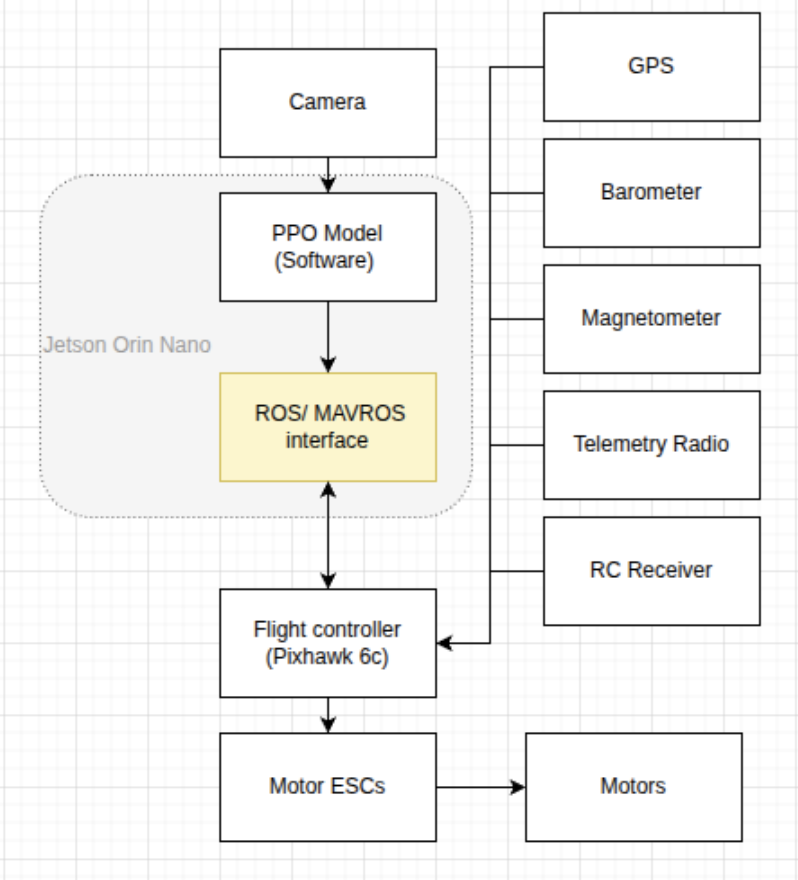
\includegraphics[width=0.85\textwidth]{figures/ros2_pipeline.png}
    \caption{ROS2 onboard data pipeline. The camera stream and Pixhawk sensor data are combined by the inference node, which runs the PPO policy and publishes velocity commands back to the Pixhawk via MAVLink.}
    \label{fig:ros2_pipeline}
\end{figure}

\subsubsection{Preparation --- The software setup}

The trained PPO policy was converted from PyTorch to TensorRT before deployment, bringing inference latency down to 20--30\,ms on the Jetson, fast enough for the 30\,Hz control loop. Velocity commands from the inference node are sent to the Pixhawk via MAVLink using MAVSDK-Python, which executes them in altitude control mode. A QGroundControl ground station on a laptop handled telemetry monitoring and safety override during all flights. Table \ref{tab:software} summarises the full software stack.

With hardware, middleware, and software aligned, the drone is ready for real-world deployment.

\begin{table}[H]
    \small
    \centering
    \caption{Software stack for training and real-world deployment.}
    \label{tab:software}
    \begin{tabular}{p{4cm} p{4cm} p{5.5cm}}
        \hline\hline
        \rowcolor{lightgray}\textbf{Component} & \textbf{Tool} & \textbf{Role} \\\hline
        Simulation environment & Cosys-AirSim + UE 5.5 & Physics, rendering, sensor simulation \\
        \rowcolor{lightlightgray} RL framework & Stable-Baselines3 + PyTorch & PPO training \\
        Image processing & OpenCV & CLAHE preprocessing, image capture \\
        \rowcolor{lightlightgray} Camera interface & ROS2 & Arducam frame streaming to Jetson \\
        Sensor interface & MAVROS & Pixhawk IMU/GPS data to Jetson \\
        \rowcolor{lightlightgray} Flight commands & MAVSDK-Python + MAVLink & Velocity commands to Pixhawk \\
        Inference optimisation & TensorRT & Real-time policy inference on Jetson \\
        \rowcolor{lightlightgray} Ground station & QGroundControl & Telemetry monitoring, safety override \\
        \hline
    \end{tabular}
\end{table}


\subsubsection{Testing --- Real world}

Real-world trials were conducted in a forest clearing under controlled weather conditions: wind speed below 3\,m/s, no precipitation, temperature 10--25\textdegree{}C, and daylight. Battery charge was maintained at 80--100\% at the start of each flight. Tree spacing was measured and marked on the ground prior to each session to match the simulation configurations exactly \cite{Loquercio2019,Jang2024}.

The same 50 flights per condition were conducted as in simulation, across identical configurations: sparse (6\,m), medium (4\,m), and dense (2\,m) tree spacing. An obstacle was counted as avoided if the tree entered the 6\,m detection corridor, no physical contact occurred, and the drone maintained forward progress. Collision detection was determined by an accelerometer spike on the Pixhawk IMU exceeding a predefined threshold. Any flight requiring manual RC failsafe activation was recorded as a failure \cite{Azzam2024}. Table \ref{tab:data_structure} retains the same data structure for real-world trials as for simulation.

\subsubsection{Testing --- Sim-to-real transfer}

Transfer efficiency is computed for each matched condition as:
\begin{equation}
    \text{Transfer Efficiency (\%)} = \frac{\text{Real-world success rate}}{\text{Simulation success rate}} \times 100
\end{equation}

A value of 100\% indicates no performance loss in transfer; lower values quantify the magnitude of the reality gap \cite{Zhao2020,Salvato2021}. This metric has been used in comparable drone RL transfer studies \cite{Loquercio2019,Azzam2024,Jang2024}. Several design decisions were specifically aimed at minimising this gap: action delay and momentum smoothing simulate real motor lag \cite{Zhao2020,Salvato2021}; Gaussian noise injection replicates physical camera sensor noise \cite{Loquercio2019}; and the simulated sensor parameters exactly match the Arducam IMX477, following the hardware-matching strategy of Kabas \cite{Kabas2022} and Loquercio et al.\ \cite{Loquercio2019}.

\end{document}
